\documentclass[11pt]{article}
\usepackage[UTF8]{ctex}
\usepackage{picinpar,graphicx,bm}
\usepackage{booktabs}
\usepackage{diagbox}
\usepackage{float}
\usepackage{setspace}
\usepackage{multirow}
\usepackage{caption}

\newcommand{\upcite}[1]{\textsuperscript{\textsuperscript{\cite{#1}}}}

% used to demo bracket for array
\usepackage{amsmath}

\usepackage{listings}
\usepackage{xcolor}
% 定义可能使用到的颜色
\definecolor{CPPLight}  {HTML} {686868}
\definecolor{CPPSteel}  {HTML} {888888}
\definecolor{CPPDark}   {HTML} {262626}
\definecolor{CPPBlue}   {HTML} {4172A3}
\definecolor{CPPGreen}  {HTML} {487818}
\definecolor{CPPBrown}  {HTML} {A07040}
\definecolor{CPPRed}    {HTML} {AD4D3A}
\definecolor{CPPViolet} {HTML} {7040A0}
\definecolor{CPPGray}  {HTML} {B8B8B8}
\lstset{
    columns=fixed,    
   % numbers=left,                                        % 在左侧显示行号
    frame=none,                                          % 不显示背景边框
    backgroundcolor=\color[RGB]{245,245,244},            % 设定背景颜色
    keywordstyle=\color[RGB]{40,40,255},                 % 设定关键字颜色
    numberstyle=\footnotesize\color{darkgray},           % 设定行号格式
    commentstyle=\it\color[RGB]{0,96,96},                % 设置代码注释的格式
    stringstyle=\rmfamily\slshape\color[RGB]{128,0,0},   % 设置字符串格式
    showstringspaces=false,                              % 不显示字符串中的空格
    language=c++,                                        % 设置语言
    morekeywords={alignas,continute,friend,register,true,alignof,decltype,goto,
    reinterpret_cast,try,asm,defult,if,return,typedef,auto,delete,inline,short,
    typeid,bool,do,int,signed,typename,break,double,long,sizeof,union,case,
    dynamic_cast,mutable,static,unsigned,catch,else,namespace,static_assert,using,
    char,enum,new,static_cast,virtual,char16_t,char32_t,explict,noexcept,struct,
    void,export,nullptr,switch,volatile,class,extern,operator,template,wchar_t,
    const,false,private,this,while,constexpr,float,protected,thread_local,
    const_cast,for,public,throw,std,size_t,__global__,__device__,__host__},
    emph={map,set,multimap,multiset,unordered_map,unordered_set,
    unordered_multiset,unordered_multimap,vector,string,list,deque,
    array,stack,forwared_list,iostream,memory,shared_ptr,unique_ptr,
    random,bitset,ostream,istream,cout,cin,endl,move,default_random_engine,
    uniform_int_distribution,iterator,algorithm,functional,bing,numeric,},
    emphstyle=\color{CPPViolet}, 
    frame=shadowbox,
    basicstyle=\footnotesize\ttfamily,
    tabsize=4,
}
\newcommand{\tabincell}[2]{\begin{tabular}{@{}#1@{}}#2\end{tabular}}


%layout
\usepackage{calc} 
\setlength\textwidth{7in} 
\setlength\textheight{9in} 
\setlength\oddsidemargin{(\paperwidth-\textwidth)/2 - 1in}
\setlength\topmargin{(\paperheight-\textheight -\headheight-\headsep-\footskip)/2 - 1.5in}


\title{《计算机图形学》读书报告  \begin{large} \hspace{5pt}——— \hspace{5pt}  渲染技术中的优化调研\end{large} }
\author{11821095 葛林林}
\begin{document}
\maketitle
\section{引言}
渲染或称为图像合成技术是一种利用2D或者3D模型自动生成具有真实感或非真实感图片的过程。在渲染技术中最核心的技术是光线跟踪技术。由于每根光线都需要对其他所有物体进行检测和进行求交运算,因此光线跟踪技术是非常耗时的。常用的几种速度优化方案有:(1)使用更快的机器;
(2)使用并行处理的方法;(3)使用更为有效的算法(例如分割物体或者分割空间);(4)减少光束个数。

虚拟场景的要素有:(1)几何信息;(2)视角;(3)纹理信息;(4)光照信息;(5)阴影信息。

\par 如何评价加速结构:(1)构建的速度;(2)使用的内存大小;(3)遍历结构的速度。


\section{并行加速方案}
2009年C. Lauterbach和M. Garland等人在线性层次包围盒的基础上针对GPU并行功能提出了基于启发式表面区域(SAH)的方案\upcite{LBVH}。在该方法中,使用多个内核来并行运行多个节点拆分尽可能使用数据并行计算单元在处理器中加速SAH评估以及实际的拆分操作。

\begin{itemize}
\item[(1)]{\bm{构建工作队列}} \mbox{}\\
在自上而下的构造过程中,由于每一个拆分操作都是完全独立的,将所有的拆分操作在多个并行核中执行是一种最简单的方式来加快速度。在这个过程中需要引入一个队列来管理拆分操作。然而GPU当前的架构并不支持实现全局工作队列。因此在该文中,提出了使用迭代的方法来并行处理所有当前工作状态的拆分并记录新的拆分操作,之后在其间对队列进行维护,从而给下一步提供一个可用的队列。	如下图所示是工作队列的构建步骤示意图:
\begin{figure}[H]
\begin{center}
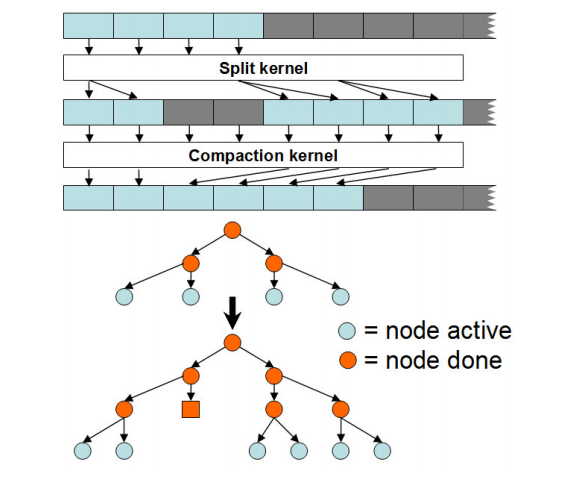
\includegraphics[scale=0.7]{SAH1.png}
\caption{工作队列的构建,通过使用两个工作队列,可以并行运行所有激活的拆分操作。 由于拆分内核可能不会输出新的拆分,因此每次拆分步骤之后会进行压缩操作来删除队列中的空白空间。}
\end{center}
\end{figure}
\item[(2)]{\bm{数据并行处理}} \mbox{}\\
为对象层次结构执行SAH拆分操作包括两个步骤:
\begin{itemize}
\item{通过评估SAH确定最佳分割位置;}
\item{基元的重排序,与kd-tree等空间分区方法不同,重排序不需要额外的内存。}
\end{itemize}
上述两个步骤都可以通过利用数据并行性和使用常见的并行操作来执行,并且每个拆分操作都在一个核上执行。
\item[(3)]{\bm{细小拆分操作的优化}} \mbox{}\\
针对由于层次结构的顶层初始拆分阶段缺乏并行性以及在最后存在很多的细小拆分导致的算法速度瓶颈问题。
本文中使用每个处理器的本地内存来维护所有的本地工作队列。由于cache非常快,从而较少了内存访问等待时间。除此之外,内核中使用尽可能少的线程来最大化利用向量运算。 分割为“小”的基元的阈值取决于可以将多少几何数据存储到本地存储器中。

\end{itemize}




\section{基于深度控制的优化方案}
1983年Hall, Roy A.和Donald P. Greenberg\upcite{Hall}等人提出了一种自适应深度的方法来减少光束的数量。
他们将光线跟踪的分为四个步骤:(1)给物理环境建模;(2)对光线在环境中的传播进行仿真;(3)确定成像平面的密度函数;(4)将离散成像平面密度信息转化为可显示的形式。
\par 传统上,任何采样点的交叉树被构造成预先指定的任意深度以确保能够捕获足够的与产生的图片相关的反射和折射信息。然而对于大多数典型环境,由反射或者透明表面组成的场景占比很少。因此有很大的空间去优化树的的深度。
\par 该文中将交点树中任何节点的贡献值的上界近似为最终采样点的颜色值,通过考虑树种每个节点的强度来使得强度达到最大。第一个节点在树上将贡献100%的最终颜色样本点。子节点的最大贡献值可以通过将代表反射孩子节点设置统一为$I_r$和$F_r$,将传输的孩子节点设置统一为$I_t$和$F_t$,最终算出相关的贡献率。可以对树中任何父节点的子节点重复此过程。 通过乘以近似最大贡献,可以计算子节点对样本点的最大累积贡献。因此,通过建立截止贡献阈值,从而可以在光线跟踪过程中自适应地控制树的深度。

\section{Hank Weghorst等人改进方案}
1984年Hank Weghorst等人\upcite{Hank}指出了一些光线跟踪的改进方案。


\begin{itemize}
\item[(1)]{\bm{包围盒的选取:}}该文中指出包围盒的选择需要考虑多种因素,如基的选取、空白投影面积等。
\item[(2)]{\bm{建立基于环境的层次结构}}
\item[(3)]{\bm{预处理}}:
由于可见表面必然与观察者最为接近,该文中借鉴了Z-buffer算法的方法产生Item Buffer,从而对物体的前后顺序得到一种索引列表,随后光线跟踪算法便可以更具该索引列表得到第一个光线交点,从而改进光线跟踪中求交的速度。
\end{itemize}

如在自适应深度控制一节中所提到的,通过使用该技术,射线树的平均深度可以小于2。 这意味着在找到第一个交叉点时执行了大部分工作。 Weghorst建议使用修改的Z缓冲算法来确定第一次命中。 将对场景进行预处理,生成的z缓冲区存储指向相交对象的指针。 然后光线追踪将从那一点开始。
\par 他表明,结合上述三种技术(自适应深度控制,分层边界体积和首次加速加速)大大减少了复杂场景的交叉计算时间。 请注意,他使用球体作为边界体积。 通常,计算改进与场景复杂性成反比。
\par Weghorst表明,结合上述三种技术(自适应深度控制,分层边界体积和首次加速加速)大大减少了复杂场景的交叉计算时间。 请注意,他使用球体作为边界体积。 通常,计算改进与场景复杂性成反比。

\section{基于层次包围盒(BVH)的改进方法}
我们将对象组包含在分层边界体积集中,并首先测试与边界体积的交集,然后仅在有交叉点的情况下对着体积所包围的对象进行测试。
\par 边界体积应易于测试交叉点,例如球体或盒子(平板)。 最佳边界体积将由底层对象的形状决定。 例如,如果对象是长而薄的,那么球体将主要包围空白空间并且盒子要好得多。 对于分层边界卷,框也更容易。使用这样的分层系统(假设它已经仔细完成)会将交叉点计算时间从对象数量的线性依赖性改变为线性和逻辑关系之间的某种程度。 这是因为,对于一个完美的情况,每个求交测试会将可能性划分为两个,并且我们将具有二叉树类型结构。
\subsection{基本概念}
\subsubsection{BVH}
边界体积层次结构(BVH)已广泛存在用于光线跟踪和碰撞检测。在交互式光线跟踪领域中,基于对象层次结构的方法由于Kd-Tree技术在CPU和GPU上得到了发展而重新获得关注。早期的方法使用简单的更新技术来维护动态数据集并且使用快速构建技术来重建BVH\upcite{LBVH}。

\subsubsection{LBVH}
2009年Lauterbach等人引入了BVH构造算法,该算法基于在场景边界框内运行的填充莫顿曲线对基元进行排序。空间填充曲线长期以来一直用于改进空间算法。可以计算沿着$n$阶莫尔顿曲线的三维点的坐标,也称为其莫顿码,将其坐标离散化为$n$位并交织它们的二进制数,从而获得$3n$位索引。 由于算法将构建层次结构的问题转化为沿曲线排序一组点的问题,Lauterbach等人将其称为线性边界体积层次(LBVH)算法。

\subsubsection{表面积启发式算法(SAH)}
SAH英文全称surface area heuristic,中文称为表面积启发式算法,表面积启发式算法法基于的理论是复杂度成本分析和概率论,主要用于解决怎样划分轴的问题,可以被应用到适用于多种类型的分层加速结构。


\subsubsection{莫顿码(Morton Code)简介}
莫顿码是一种将量化的n维向量映射为整数标量值的方法。莫顿码引入空间填充曲线,它提供了一种稳定的量化矢量的稳定排序方法,这意味着具有相同子序列莫顿码的矢量在空间上是彼此接近。虽然有其他形式的空间填充曲线,但是莫顿码计算的简单性使得它得到了广泛的运用。莫顿码可以通过几次简单的比特交叉操作得到。如下图所示是二维莫顿码的简单示例:
\begin{figure}[H]
\begin{center}
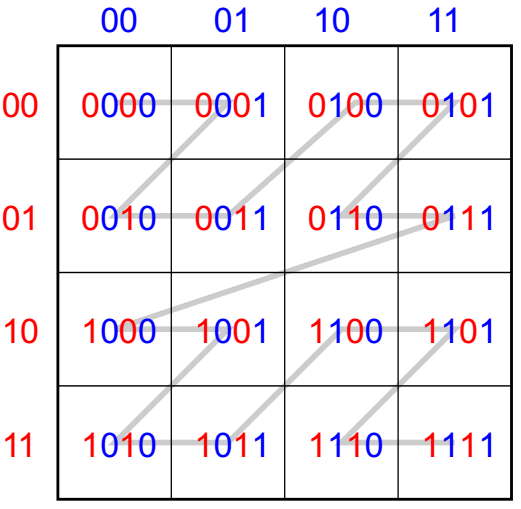
\includegraphics[scale=0.4]{morton-code.png}
\caption{二维莫顿码示意图}
\end{center}
\end{figure}

\par 莫顿码的一个主要参数是该码的位数。莫顿码的产生步骤如下:
\begin{itemize}
\item[(1)]{\bm{确认量化坐标}}:例如对应三维的莫顿码其量化坐标为$\bm{v}^{*}=\{v_x^{*},v_y^{*},v_z^{*}\}$

\item[(2)]{\bm{交叉操作}}:例如对应的三维莫顿码,假设量化坐标$v_x^{*}=x_7x_6x_5x_4x_3x_2x_1x_0$,$v_y^{*}=y_7y_6y_5y_4y_3y_2y_1y_0$,$v_z^{*}=z_7z_6z_5z_4z_3z_2z_1z_0$,利用交叉操作得到的莫顿码为
$$
m(v^{*})=x_7y_7z_7x_6y_6z_6x_5y_5z_5x_4y_4z_4x_3y_3z_3x_2y_2z_2x_1y_1z_1x_0y_0z_0
$$
\end{itemize}
查表法可用于预先计算某些位范围的代码,然后在运行时通过简单的添加和组合进行组合。

\subsection{基于LBVH的方法}
2009年C. Lauterbach和M. Garland等人提出了线性层次包围盒\upcite{LBVH}。



\subsection{基于HLBVH的方法}
2010年J. Pantaleoni和D. Luebke提出了HLBVH方法\upcite{HLBVH}。涉及到的主要技术有\bm{莫顿码构建线性层次包围盒}、surface area heuristic、

\subsection{基于STBVH的方法}
Sven Woop、Attila T. Áfra和Carsten Benthin等人提出了时空层次包围盒的方法\upcite{STBVH}。

\subsection{基于扩展莫顿码的BVH方法}
2017年Marek Vinkler、Jiri Bittner和Vlastimil Havran\upcite{accelerator2}等人在莫顿码的基础上进行扩展,从而在提高BVH构造结果的同时不会引起计算量的增加。
\par 该文中对针对硬件的加速方法做出了分析。第一个利用多核CPU加快构建高质量数据结构的重要技术由Havran等人在2006年提出binned BVH\upcite{cpus1}。

\subsubsection{扩展莫顿码(Extended Morton Code)}
扩展莫顿码在莫顿码的基础上做了如下的改进
\begin{itemize}
\item[(1)]{\bm{加入对象大小编码}}
由于对象之间大小差异巨大会影响对象聚类的结果,所以讲对象的大小进行编码加入莫顿码。则三维的莫顿码示例如下:
$$(x,y,z,s)$$
其中$x,y,z$代表几何基元的中心位置,$s$代表几何基元的大小。该大小$s$是归一化的大小,使得使用给定位数表示的最高值对应于场景边界框的对角线,如下图所示是对基元的大小进行编码的效果图:
\begin{figure}[H]
\begin{center}
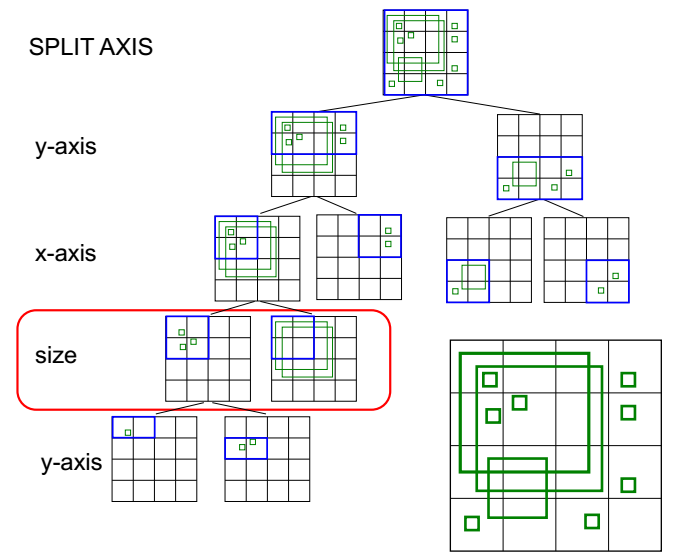
\includegraphics[scale=0.6]{EMC.png}
\caption{基元大小编码效果图,其中size部分能够将大小相差较大的部分分开来}
\end{center}
\end{figure}
\item[(2)]{\bm{减少物体尺寸编码的位数}}
主要思想是每七位加入一位尺寸位,使得每个轴进行两次分割。

\item[(3)]{\bm{自适应轴顺序}}
由于不同空间轴相对性的比特位的顺序会影响BVH的质量,因此在EMC中首先先分割最大轴。

\item[(4)]{\bm{}}

\end{itemize}




\begin{thebibliography}{3}
\bibitem{Hall} Hall, Roy A., and Donald P. Greenberg. "A testbed for realistic image synthesis." IEEE Computer Graphics and Applications 3.8 (1983): 10-20.

\bibitem{Hank}Weghorst, Hank, Gary Hooper, and Donald P. Greenberg. "Improved computational methods for ray tracing." ACM Transactions on Graphics (TOG) 3.1 (1984): 52-69.



\bibitem{accelerator3} Woop, Sven, Attila T. Áfra, and Carsten Benthin. "STBVH: a spatial-temporal BVH for efficient multi-segment motion blur." Proceedings of High Performance Graphics. ACM, 2017.

\bibitem{accelerator4} Vinkler, Marek, Jiri Bittner, and Vlastimil Havran. "Extended Morton codes for high performance bounding volume hierarchy construction." Proceedings of High Performance Graphics. ACM, 2017.

\bibitem{cpus1} Havran, Vlastimil, Robert Herzog, and Hans-Peter Seidel. "On the fast construction of spatial hierarchies for ray tracing." Interactive Ray Tracing 2006, IEEE Symposium on. IEEE, 2006.

\bibitem{LBVH} Lauterbach, Christian, et al. "Fast BVH construction on GPUs." Computer Graphics Forum. Vol. 28. No. 2. Oxford, UK: Blackwell Publishing Ltd, 2009.

\bibitem{HLBVH} Pantaleoni, Jacopo, and David Luebke. "HLBVH: hierarchical LBVH construction for real-time ray tracing of dynamic geometry." Proceedings of the Conference on High Performance Graphics. Eurographics Association, 2010.

\bibitem{STBVH} Woop, Sven, Attila T. Áfra, and Carsten Benthin. "STBVH: a spatial-temporal BVH for efficient multi-segment motion blur." Proceedings of High Performance Graphics. ACM, 2017.

\bibitem{accelerator2} Benthin, Carsten, et al. "Improved two-level BVHs using partial re-braiding." Proceedings of High Performance Graphics. ACM, 2017.



\end{thebibliography}
\end{document} 
\end{document}
